\section*{Goal of the Thesis}
General relativity has passed every current precision test in the weak-field regime, while the strong-gravity and high-curvature regimes remain active frontiers. Black-hole binary dynamics, scattering observables, and gravitational radiation are central probes of this regime. Modern collider-inspired methods, especially scattering amplitudes and effective field theory (EFT), now provide a systematic and highly efficient route to compute classical observables that are difficult to obtain using traditional approaches alone.

The broad objective of this thesis is to explore these methodologies in the context of beyond General Relativity:
\begin{enumerate}
\item Classical two-body dynamics in gravity,
\item Amplitude and worldline-based computational frameworks, and
\item Eikonal amplitudes in modified gravity and implication to celestial holography.
\end{enumerate}
The focus is on effective theories of gravity and departures from Einstein gravity, where new interactions can leave signatures in conservative, and radiative dynamics as well as more formal aspects like flat space holography.
\section{Context and Motivation}
The detection of gravitational waves (GWs) \cite{LIGOScientific:2016aoc, LIGOScientific:2016sjg, LIGOScientific:2016vlm, LIGOScientific:2017bnn, Kokeyama:2020dkg, LIGOScientific:2019hgc} has opened a powerful new pathway to test gravity. Alongside its remarkable success in describing the dynamics of spacetime and underpinning our current picture of the Universe’s large-scale structure, Einstein’s theory can now be confronted directly with strong-field, time-dependent data from compact-object sources. Gravitational waves are produced most prominently by compact binaries involving black holes and neutron stars, and the ability to detect these signals motivates increasingly high-precision computations of the source dynamics. The evolution of such a binary is commonly separated into three stages: the \textit{inspiral}, \textit{merger}, and \textit{ringdown}. Probing the merger regime---where gravity is genuinely strong and highly non-linear---typically requires non-perturbative techniques based on numerical relativity \cite{Gourgoulhon:2012,Lehner:2014asa, LIGOScientific:2014oec}.
\par
Beyond quasi-circular inspirals, compact objects can also undergo astrophysical scattering encounters on hyperbolic trajectories; the associated burst-like radiation provides complementary access to source properties and can be used to place constraints on theory parameters. In this broader landscape, it is notable that Quantum Field Theory (QFT), originally developed to describe interactions among subatomic particles, has emerged as an efficient and systematically improvable toolkit for analytic computations in the weak-to-intermediate field regimes relevant to both inspiral and scattering dynamics.
\noindent
\section*{Why Go Beyond General Relativity?}
%\onehalfspacing
Despite its remarkable empirical success, General Relativity (GR) is widely regarded as an incomplete framework. By construction, it is a classical field theory governing the gravitational interactions of macroscopic objects. However, like all other fundamental forces in nature, gravity must ultimately be reconciled with quantum theory. Because GR is not ultraviolet (UV) complete, it breaks down at extremely high energies or vanishingly short distances, indicating an absolute need for new physics. As Steven Weinberg pointed out, Einstein's gravity is best viewed not as the final, fundamental theory of nature, but as the leading term in a low-energy effective description. This perspective strongly motivates the study of \emph{effective field theories (EFTs) of gravity}. In an EFT framework, standard GR is augmented by higher-derivative operators that capture the low-energy imprints of high-energy dynamics. The effective action takes the form of an infinite derivative expansion:
\begin{equation}
    S = \int d^4x \sqrt{-g} \left( c_1 R + c_2 \mathcal{R}^2 + c_3 \mathcal{R}^3 + \cdots \right)
\end{equation}
where the leading-order term $R$ is the standard Ricci scalar. From the second order onwards, $\mathcal{R}^n$ schematically represents all possible combinations of curvature invariants (e.g., $R_{\mu\nu}R^{\mu\nu}$ or $R_{\mu\nu\rho\sigma}R^{\mu\nu\rho\sigma}$) at a given derivative order. Each successive term in this expansion probes increasingly smaller length scales, predicting deviations from GR that can be used to build phenomenological models. 

Truncating this expansion at the next-to-leading order yields the simplest non-trivial extension of GR: quadratic gravity,
\begin{equation}
     S_{g}=\int d^4 x \sqrt{-g}\left(\kappa \,{R}+\alpha {R}_{\mu\nu}{R}^{\mu\nu}-\frac{1}{3}(\alpha+\beta){R}^2\right).
\end{equation}
The inclusion of curvature-squared contributions in classical gravity was first proposed by Weyl \cite{weyl}, and their ability to render gravity power-counting renormalizable was subsequently demonstrated \cite{1962JMP.....3..608U, PhysRevD.16.953}. However, this favourable UV behaviour comes at a cost. At the level of the tree-level propagator \eqref{3.2h}, the UV behaviour improves from a $1/q^2$ to a $1/q^4$ fall-off, but this modification unavoidably introduces a massive spin-2 ghost with mass $m = \sqrt{\kappa/\alpha}$. To quantise the theory such that all excitations have positive-definite energy, one must introduce negative-norm states into the Hilbert space, which typically signals a breakdown of perturbative unitarity \cite{PhysRev.79.145}. Consequently, the physical consistency of higher-derivative gravity remains highly contested. Yet, as emphasised by  Fradkin and  Tseytlin \cite{FRADKIN1982469}, unitarity is fundamentally a dynamical property. It cannot be definitively assessed at the tree level or within a strictly perturbative regime; a complete picture requires accounting for loop corrections and non-perturbative radiative effects. 


Moreover, GR leaves major puzzles in fundamental physics and cosmology unresolved, such as the origin of dark energy and the exact nature of spacetime singularities, further reinforcing the perspective that Einstein gravity is merely the leading term in a broader effective description. Introducing higher-curvature invariants into the action is theoretically sound, provided that diffeomorphism invariance is rigorously preserved. As suggested by our previous discussion, the impact of these higher-derivative operators becomes highly pronounced in strong-gravity regimes, such as the immediate vicinity of merging black holes. At the classical level, the dimensionful couplings associated with these terms introduce characteristic length scales that dictate exactly when and where these deviations from standard GR become physically significant. Furthermore, upon linearization, higher-derivative terms typically induce new dynamical degrees of freedom beyond the standard massless spin-2 graviton, signaling a fundamental departure from pure GR dynamics. 

Beyond bottom-up phenomenological models, effective field theories can also be constructed via top-down approaches when a complete UV theory is specified. String theory, a premier candidate for a consistent theory of quantum gravity, perfectly exemplifies this paradigm. When deriving the low-energy effective action of string theory, higher-derivative curvature operators naturally and inevitably emerge. Alongside these operators, this top-down derivation universally predicts the presence of additional dynamical degrees of freedom, such as the scalar dilaton and various gauge fields and higher form fields (e.g the Einstein-Dilaton-Higher form theory \cite{Hassan:1991mq}), which further enrich the gravitational sector.
\par
This thesis is primarily devoted to the calculation of \emph{observable} quantities within such effective theories of gravity (in both astrophysical scenarios: inspiral and scattering), with particular emphasis on higher-derivative extensions and related modifications that become relevant in scattering or inspiral processes. Using modern amplitude-based and worldline-QFT(and EFT) techniques, we compute conservative and radiative observables (such as impulse, scattering angle, and waveform) in regimes where precision is essential and where deviations from Einstein gravity can leave measurable imprints.

\section{Quantum Field Theory and its Classical Limit}
In standard undergraduate and graduate presentations of quantum field theory, one often learns that the perturbative expansion of scattering amplitudes may be viewed both as an expansion in the coupling constants and as an expansion in the Planck constant $\hbar$. Within this perspective, tree-level amplitudes, of order $\hbar^{0}$, are identified with the classical result, while higher-loop contributions are interpreted as quantum corrections. While this intuition is often useful, it is not entirely general and can be misleading in certain situations.
This conventional picture is primarily based on particle-physics applications, where the external states are genuinely quantum particles with momenta scaling as
\(k^\mu=\hbar\,\bar{k}^\mu\),
where $\bar{k}^\mu$ is the associated wave vector. With this scaling, the $\hbar$-counting of amplitudes provides a natural way to distinguish classical from quantum effects. However, when quantum field theory is employed to study the scattering of macroscopic compact objects such as black holes or neutron stars, the situation is qualitatively different. These external states correspond to classical bodies, and their momenta do not scale with $\hbar$ in the same manner. One is then led to an important conceptual question: how does one isolate the classical content of a quantum field theoretic amplitude when the external particles are themselves classical objects? Over the past couple of decades, substantial conceptual and computational advances have emerged to address this question. Let us discuss the seemingly different approaches in this context.

\vspace{0.5 cm}
\thesisleadtopic{PM Expansion of Amplitudes \cite{Holstein:2004dn,Bern:2019crd,Bern:2020buy,Bern:2019nnu,Bern:2020gjj,Bern:2021dqo,Bern:2021xze,Bern:2022kto,Bern:2025zno,Bjerrum-Bohr:2002aqa,Bjerrum-Bohr:2021wwt}:}
In scattering processes involving black holes with velocities comparable to the speed of light, the usual post-Newtonian (PN) expansion, which is fundamentally a low-velocity expansion and is well suited to the inspiral regime, ceases to be a good approximation. In such situations, it is more appropriate to employ the \emph{post-Minkowskian} (PM) expansion, which is organised as an expansion in Newton's constant $G$ while retaining the full velocity dependence. Since relativistic scattering amplitudes are naturally arranged as a perturbative series in $G$, keeping all orders in velocity, one defines the PM potential as
\begin{equation}
V(\boldsymbol{p},\boldsymbol{r})=\sum_{n=1}^\infty \left(\frac{G}{|\boldsymbol{r}|}\right)^n c_n(\boldsymbol{p}^2)\, ,
    \label{1.2}
\end{equation}

where the coefficients $c_n(\boldsymbol{p}^2)$ are functions of $\boldsymbol{p}^2 \sim \boldsymbol{v}^2$ and therefore encode arbitrarily high powers of the velocity.


To extract genuinely new information in PM dynamics that can be incorporated into gravitational-wave templates, however, one must carefully understand how scattering data encode the conservative two-body dynamics. The central idea underlying the connection between scattering amplitudes and the bound orbit motion of compact binaries is that both are governed by the same underlying theory, or more precisely, by the same classical effective potential. Thus, by construction, the effective two-body potential in \eqref{1.2} reproduces the same long-range classical physics as the full gravitational theory for kinematics specified by the masses and velocities of the scattering bodies. It then becomes possible to use scattering amplitudes as a tool to determine the effective potential. It was demonstrated long ago that modern field-theoretic methods are particularly powerful for computing scattering amplitudes relevant to such classical problems \cite{Holstein:2004dn}. As emphasised earlier, the main objective of this program is to systematically isolate the classically relevant part of quantum scattering amplitudes.

Let us begin by specifying the theory. A pair of gravitationally interacting spinless compact objects with masses $m_1$ and $m_2$ may be modelled by real scalar fields and described by the action below, neglecting finite-size corrections and spin:
\begin{equation}
        S=\int d^4x \sqrt{-g}\,R
        +\frac{1}{2}\sum_{i=1}^2 \int d^4x \sqrt{-g}\,
        \left(D_\mu \phi_i D^\mu \phi_i - m_i^2 \phi_i^2\right)\, .
\end{equation}
Here, one neglects direct interactions between the scalar fields $\phi_i$, consistent with the classical assumption that the two objects remain widely separated and interact only through gravity.

For conservative scattering, one considers the process in which $\phi_1$ and $\phi_2$ scatter elastically. In the center-of-mass frame, the incoming momenta are $(E_1,\boldsymbol{p})$ and $(E_2,-\boldsymbol{p})$, while the outgoing momenta are $(E_1,\boldsymbol{p}')$ and $(E_2,-\boldsymbol{p}')$. The momentum transfer is then
\begin{equation}
    q=(0,\boldsymbol{q})=(0,\boldsymbol{p}-\boldsymbol{p}')\, .
\end{equation}
The classical regime is characterized by an impact parameter much larger than the de Broglie wavelength, $ |\boldsymbol{b}| \gg \lambda = \frac{1}{|\boldsymbol{p}|}\,,$ or equivalently, by an orbital angular momentum parametrically large compared to $\hbar$, in accordance with the Bohr correspondence principle:
\begin{equation}
    J \gg \hbar \qquad (\text{equivalently, setting }\hbar=1:\; J\gg 1)\, .
\end{equation}
Physically, the condition $J\gg 1$ means that the impact parameter is large compared to the de Broglie wavelength, so that the scattering process admits a semiclassical description.

In this regime, the momentum transfer $q$ is small compared to the hard external scales set by the Mandelstam invariants and the particle masses. The classical contributions then arise from the non-analytic, long-distance dependence of the amplitude on
\begin{equation}
t=q^2\, .
\end{equation}
More precisely, we have a scale hierarchy
\begin{equation}
    s,\; |u|,\; m_i^2 \sim J^2 |t| \gg |t| = |q|^2\, ,
\end{equation}
so that an expansion at large $J$ is equivalent to an expansion in small $|q|$. This is what we refer to as the \emph{soft expansion}: an expansion about small momentum transfer while keeping the hard external kinematics fixed. Within this expansion, the classical part of the amplitude can be systematically isolated, for instance as the leading terms in $|q|$ at fixed $s$ and fixed masses. It is useful to distinguish three classical limits, depending on the degree of relativistic motion:
\begin{equation}
\begin{split}
    &\textrm{Generic classical limit:} \qquad\qquad\qquad\;\; J \gg 1, \textrm{expansion in } \mathcal{O}(|\boldsymbol{q}|)\\
    &\textrm{Near-static (PN) classical limit:} \qquad\,\,\, J \gg 1,\;\; \sigma \sim 1,\\
    &\textrm{High-energy classical limit:} \qquad\qquad\;\; J \gg 1,\;\; \sigma \gg 1,
\end{split}
\end{equation}
where the boost parameter is defined as $ \sigma \equiv \frac{k_1\!\cdot\! k_2}{m_1 m_2}\, .$
This parameter measures the relative velocity of the two bodies: $\sigma \simeq 1$ corresponds to the near-static, post-Newtonian regime, whereas $\sigma \gg 1$ describes ultra-relativistic scattering. In the latter case, the hierarchy of scales becomes even stronger,
\begin{equation}
    s,\; |u| \gg m_i^2 \sim J^2 |t| \gg |t| = |q|^2\, .
\end{equation}
Classical considerations also impose important restrictions on the class of Feynman diagrams that can contribute to the scattering amplitude. These constraints may be summarised as follows (see \cite{youtube_484KUavMo0}):
\begin{itemize}[leftmargin=2em,itemsep=1.2em,topsep=0.6em]

\item
\begin{minipage}[t]{0.64\linewidth}
Any relevant Feynman loop diagram must contain at least one matter line in the loop; in particular, purely messenger loops are excluded from the classical analysis.
\end{minipage}\hfill
\begin{minipage}[t]{0.4\linewidth}
\vspace{-10.3pt}
\hspace{2 cm}
\centering
\includegraphics[width=\linewidth]{FD3.png}
\end{minipage}

\item
\begin{minipage}[t]{0.64\linewidth}
Diagrams with intersecting matter lines are also excluded. Classically, this is understood as a consequence of the large-separation regime, in which the two bodies do not undergo a head-on collision.
\end{minipage}\hfill
\begin{minipage}[t]{0.4\linewidth}
\vspace{-10.3pt}
\centering
\includegraphics[width=\linewidth]{FD.png}
\end{minipage}
\item
\begin{minipage}[t]{0.64\linewidth}
For lower loop orders, in particular for $L\leq 2$, messenger lines that begin and end on the same matter line do not contribute to the conservative potential. More precisely, diagrams of this type do not enter the conservative dynamics at one and two loops. At two loops, however, they may contribute to the radiative or dissipative sector when the appropriate propagator momenta are taken to be soft and on shell. At higher loop orders ($L\ge 3$), the situation becomes more subtle: multiple radiation lines may simultaneously go on shell, and such configurations can then contribute even to the conservative dynamics.
\end{minipage}\hfill
\begin{minipage}[t]{0.40\linewidth}
\vspace{0pt}
\centering
\includegraphics[width=\linewidth]{FD2.png}
\end{minipage}
\end{itemize}
\vspace{0.2 cm}
\thesisleadtopic{Kosower-Maybee-O'Connell (KMOC) Formalism \cite{Kosower:2018adc}.} The approach described above is physically quite intuitive: one first extracts an effective two-body potential from the scattering amplitude and then uses this potential to derive the relevant classical observables. However, the subsequent step of obtaining directly measurable quantities, such as those needed for gravitational-wave templates, is a rather different and considerably more involved problem. A major conceptual development in this direction came in 2018, when Kosower, Maybee, and O’Connell proposed a framework in which classical observables—such as the impulse, radiated momentum, and waveform—can be computed directly from scattering amplitudes, without passing through an intermediate effective potential. Although this approach will not be used in the present thesis, it is nonetheless worthwhile to review its basic ideas, since it provides a powerful and complementary perspective on the relation between quantum scattering amplitudes and classical gravitational dynamics. The KMOC formalism provides a direct route from on-shell amplitudes to classical observables, such as the impulse and radiated momentum, without first constructing an effective potential. Its main conceptual point is that the classical limit is not simply the tree-level truncation of the amplitude. Restoring $\hbar$, an $n$-point, $L$-loop amplitude scales as
\begin{equation}
    \mathcal A_{n,L}\sim \hbar^{\,1-\frac{n}{2}-L},
\end{equation}
so loop order alone does not determine whether a contribution is classical. Instead, one takes $\hbar\to0$ while keeping the massive external momenta fixed and scaling the exchanged or emitted massless momenta as $   q^\mu=\hbar\,\bar q^\mu,
    \qquad
    k^\mu=\hbar\,\bar k^\mu.$ Hence, the classical information is isolated from the soft-momentum sector of the amplitude. The incoming state is a semiclassical two-body wave packet with impact parameter $b^\mu$,
\begin{equation}
\begin{split}
    |{\rm in}\rangle_b
    &=
    \int d\Phi(p_1)\,d\Phi(p_2)\,
    \phi_1(p_1)\phi_2(p_2)\,
    e^{\,i b\cdot p_1/\hbar}\,
    |p_1,p_2\rangle, \\
    d\Phi(p)
    &=
    \hat d^4p\,\hat\delta^{(+)}(p^2-m^2),
    \qquad
    \hat d^4p\equiv \frac{d^4p}{(2\pi)^4}.
\end{split}
\end{equation}
Observables are then defined in the out-state, $ \langle \hat{\mathcal O}\rangle
    =
    {}_b\langle{\rm in}|\,S^\dagger \hat{\mathcal O} S\,|{\rm in}\rangle_b.$ For the impulse on particle $1$,
\begin{equation}
\begin{split}
    \Delta p_1^\mu
    &=
    {}_b\langle{\rm in}|\,S^\dagger \hat P_1^\mu S\,|{\rm in}\rangle_b
    -
    {}_b\langle{\rm in}|\,\hat P_1^\mu\,|{\rm in}\rangle_b
    \notag\\
    &=
    I_{(1)}^\mu+I_{(2)}^\mu.
\end{split}
\end{equation}
Here $I_{(1)}^\mu$ is linear in the amplitude, whereas $I_{(2)}^\mu$ is a quadratic unitarity (cut) contribution. Schematically,
\begin{equation}
\begin{split}
    I_{(1)}^\mu
    &\propto
    \int d\Phi(p_1)\,d\Phi(p_2)\,\hat d^4q\,
    e^{-i b\cdot q/\hbar}\,
    i q^\mu\,
    \mathcal A(p_1,p_2\!\to\! p_1+q,p_2-q), \\
    I_{(2)}^\mu
    &\propto
    \sum_X \int \cdots\,
    w_1^\mu\,
    \mathcal A\,\mathcal A^* .
    \end{split}
\end{equation}
Thus, beyond leading order, the classical impulse is an inclusive observable built from both linear and cut terms evaluated in the soft region. Radiation is treated analogously by defining
\begin{equation}
\begin{split}
    R^\mu
    =
    {}_b\langle{\rm in}|\,S^\dagger \hat K^\mu S\,|{\rm in}\rangle_b.
\end{split}
\end{equation}
In the classical limit it takes the form,
\begin{equation}
    R^\mu_{\rm cl}
    =
    \hbar^{-3}
    \sum_X \int d\Phi(k)\,K_X^\mu\,
    \big|\mathcal R(k,r_X)\big|^2 ,
\end{equation}
with the radiation kernel
\begin{equation}
\begin{split}
    \mathcal R(k,r_X)
    &=
    \hbar^{3/2}
    \prod_{i=1}^2
    \int \hat d^4w_i\,
    \hat\delta(2p_i\!\cdot w_i+w_i^2)
    \\
    &\quad\times
    \hat\delta^{(4)}(w_1+w_2-k-r_X)\,
    e^{\,i b\cdot w_1/\hbar}\,
    \mathcal A(p_1+w_1,p_2+w_2\!\to\! p_1,p_2,k,r_X).
\end{split}
\end{equation}
The KMOC formalism, therefore, extracts conservative and radiative observables directly from the $S$-matrix: the classical limit is selected by soft $\hbar$-scaling, not by loop order alone.


\thesisleadtopic{Worldline Formalisms: PM-EFT \cite{Kalin:2020mvi,Kalin:2022hph} and WQFT \cite{Mogull:2020sak,Jakobsen:2022psy}} In addition to direct methods based on scattering amplitudes, there exist complementary worldline approaches for studying the classical two-body problem. One such framework is Post-Minkowskian Effective Field Theory (\textbf{\texttt{PM-EFT}}), which is closely related to the \textbf{\texttt{PN-EFT}}/\textbf{\texttt{NRGR}} methods familiar from the post-Newtonian expansion. In this sense, PM-EFT provides a natural counterpart to the PM expansion of amplitudes discussed earlier. Another important development is Worldline Quantum Field Theory (\textbf{\texttt{WQFT}}), which in many ways complements the KMOC formalism. From the perspective of explicit computations, both PM-EFT and WQFT are especially attractive, since the relevant classical information can be extracted entirely from tree-level worldline diagrams. Put differently, one avoids the need to evaluate diagrams containing pure messenger loops.

Unlike amplitude-based approaches, in PM-EFT the black holes are modeled directly as point particles rather than scalar fields. It is convenient to write the point-particle action in Polyakov form,
\begin{equation}
       S_{\rm pm}
       =
       -\sum_{a=1,2}\frac{m_a}{2}\int d\sigma_a\, e_a
       \left(
       \frac{1}{e_a^2}\,g_{\mu\nu}(x_a)v_a^\mu v_a^\nu+1
       \right).
  \end{equation}
A useful feature of this representation is that, unlike in the usual post-Newtonian treatment, the post-Minkowskian expansion is naturally formulated using proper time to parametrise the worldlines. The conservative two-body effective action is obtained by integrating out the metric fluctuations,
\begin{equation}
    e^{iS_{\rm eff}[x_a]}
    =
    \int \mathcal{D}h_{\mu\nu}\,
    e^{\,iS_{\rm EH}[h]+iS_{\rm GF}[h]+iS_{\rm pp}[x_a,h]},
\end{equation}
and it admits an expansion in powers of Newton's constant,
\begin{equation}
    S_{\rm eff}=\sum_n \int d\tau\, L_n,
    \qquad
    L_n:\mathcal O(G^n).
\end{equation}
Once the effective action is known, classical observables such as the impulse or the deflection angle can be systematically extracted from it. In particular, the impulse on particle \(i\) is given by
\begin{equation}
    \Delta p_i^\mu
    =
    -\eta^{\mu\nu}\sum_n \int_{-\infty}^{\infty} d\tau_i\,
    \frac{\partial L_n}{\partial x_i^\nu}.
\end{equation}
Thus, PM-EFT complements the amplitude-based approach discussed previously: rather than working directly with scattering amplitudes, one reduces the problem to the computation of an effective action, or equivalently an effective potential, from which the conservative dynamics can be derived.

On the other hand, WQFT was introduced as a worldline framework closely connected in spirit to the KMOC program. As in PM-EFT, the compact objects are represented by point particles. However, unlike in standard quantum field theory, one treats not only the messenger fields but also the worldline degrees of freedom as dynamical variables. The WQFT partition function is defined as
\begin{equation}
    Z_{\textrm{WQFT}}^{(n)}
    =
    \mathcal{N}
    \int \mathcal{D}h_{\mu\nu}\,
    e^{iS_{EH}+iS_{gf}}
    \Big(\prod_{i=1}^{n}\mathcal{D}x_i\,e^{iS_{pm}^i}\Big).
\end{equation}
It was further observed that, in the appropriate regime, the WQFT partition function is related to the scattering amplitude through the eikonal phase,
\begin{equation}
    Z_{\textrm{WQFT}}^{(n)}=e^{i\chi},
\end{equation}
where \(\chi\) denotes the eikonal phase. In computing this phase one must keep track of the \(i\varepsilon\)-prescriptions of the worldline propagators. {\color{black}A naive time-symmetric/Feynman prescription may leave spurious infrared poles. Recently in \cite{Kim:2024svw}, those issues has been dealt. We will take a moment to discuss them in the next section.
\paragraph{Magnus expansion and the eikonal generator.}
The relation above should be understood as a shorthand appropriate to the elastic/eikonal sector. A more precise formulation starts from the logarithm of the unitary scattering operator. Following the recent analysis of the classical eikonal from the Magnus expansion~\cite{Kim:2024svw}, one writes
\begin{align}
    \widehat S
    =
    1+\frac{i}{\hbar}\widehat T
    =
    \exp\!\left(\frac{i}{\hbar}\widehat N\right)
    \equiv
    \exp\!\left(\frac{i}{\hbar}\widehat\chi\right),
    \qquad
    \widehat N^\dagger=\widehat N .
\end{align}
Here \(\widehat T\) is the usual transition operator, while \(\widehat N\) is the Hermitian operator appearing in the exponent. The classical eikonal is the classical limit of this logarithm, not the naive amplitude itself. This distinction separates the genuine eikonal generator from the Born iterations already generated by exponentiation. 

\begin{figure}[htb!]
\centering
\color{black}
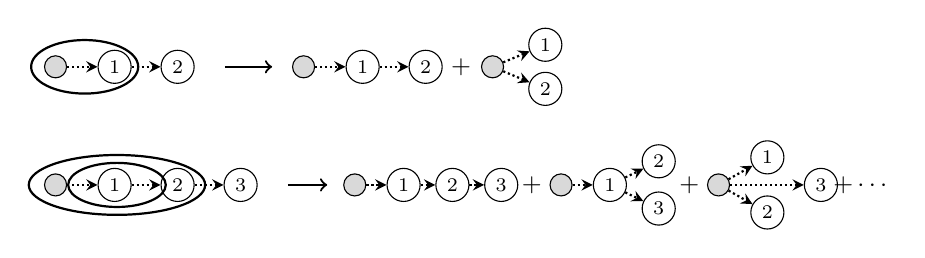
\begin{tikzpicture}[
    font=\small,
    op/.style={circle,draw=black!80!black,fill=white,inner sep=1.2pt,minimum size=0.42cm,font=\scriptsize},
    root/.style={circle,draw=black!80!black,fill=black!15,inner sep=1pt,minimum size=0.28cm},
    cut/.style={densely dotted,draw=black!80!black,thick,->,>=stealth},
    arr/.style={->,draw=black!80!black,thick}
]
    \node[root] (r0) at (0,0) {};
    \node[op] (a0) at (0.75,0) {1};
    \node[op] (b0) at (1.55,0) {2};
    \draw[cut] (r0) -- (a0);
    \draw[cut] (a0) -- (b0);
    \draw[black!80!black,thick] (0.37,0) ellipse (0.68 and 0.34);

    \draw[arr] (2.15,0) -- (2.75,0);

    \node[root] (r1) at (3.15,0) {};
    \node[op] (a1) at (3.9,0) {1};
    \node[op] (b1) at (4.7,0) {2};
    \draw[cut] (r1) -- (a1);
    \draw[cut] (a1) -- (b1);
    \node at (5.15,0) {\(+\)};
    \node[root] (r2) at (5.55,0) {};
    \node[op] (a2) at (6.22,0.28) {1};
    \node[op] (b2) at (6.22,-0.28) {2};
    \draw[cut] (r2) -- (a2);
    \draw[cut] (r2) -- (b2);

    \node[root] (s0) at (0,-1.5) {};
    \node[op] (s1) at (0.75,-1.5) {1};
    \node[op] (s2) at (1.55,-1.5) {2};
    \node[op] (s3) at (2.35,-1.5) {3};
    \draw[cut] (s0) -- (s1);
    \draw[cut] (s1) -- (s2);
    \draw[cut] (s2) -- (s3);
    \draw[black!80!black,thick] (0.78,-1.5) ellipse (1.12 and 0.38);
    \draw[black!80!black,thick] (0.78,-1.5) ellipse (0.62 and 0.28);

    \draw[arr] (2.95,-1.5) -- (3.45,-1.5);

    \node[root] (t0) at (3.8,-1.5) {};
    \node[op] (t1) at (4.42,-1.5) {1};
    \node[op] (t2) at (5.04,-1.5) {2};
    \node[op] (t3) at (5.66,-1.5) {3};
    \draw[cut] (t0) -- (t1);
    \draw[cut] (t1) -- (t2);
    \draw[cut] (t2) -- (t3);

    \node at (6.05,-1.5) {\(+\)};
    \node[root] (u0) at (6.42,-1.5) {};
    \node[op] (u1) at (7.04,-1.5) {1};
    \node[op] (u2) at (7.66,-1.20) {2};
    \node[op] (u3) at (7.66,-1.80) {3};
    \draw[cut] (u0) -- (u1);
    \draw[cut] (u1) -- (u2);
    \draw[cut] (u1) -- (u3);

    \node at (8.05,-1.5) {\(+\)};
    \node[root] (v0) at (8.42,-1.5) {};
    \node[op] (v1) at (9.04,-1.15) {1};
    \node[op] (v2) at (9.04,-1.85) {2};
    \node[op] (v3) at (9.72,-1.5) {3};
    \draw[cut] (v0) -- (v1);
    \draw[cut] (v0) -- (v2);
    \draw[cut] (v0) -- (v3);
\node at (10.22,-1.5) {\(+\cdots\)};
\end{tikzpicture}
\caption{Schematic bubble notation for nested Poisson brackets. Popping a bubble produces oriented causal cuts according to the Leibniz rule.}
\label{fig:eikonal-bubble-poisson}
\end{figure}
The operator \(\widehat N\) acts as the generator of the scattering process. For any asymptotic observable,
\begin{align}
    \widehat{\mathcal O}_{\rm out}
    =
    \widehat S^\dagger
    \widehat{\mathcal O}_{\rm in}
    \widehat S
    =
    e^{-i\widehat N/\hbar}
    \widehat{\mathcal O}_{\rm in}
    e^{i\widehat N/\hbar}.
\end{align}
Taking the classical limit turns commutators into Poisson brackets,
\begin{align}
    \frac{1}{i\hbar}
    [\widehat A,\widehat B]
    \longrightarrow
    \{A,B\}_{\rm PB},
\end{align}
so that
\begin{align}
    \mathcal O_{\rm out}
    =
    e^{\{N_{\rm cl},\,\cdot\,\}_{\rm PB}}
    \mathcal O_{\rm in}
    =
    \mathcal O_{\rm in}
    +
    \{N_{\rm cl},\mathcal O_{\rm in}\}_{\rm PB}
    +
    \frac{1}{2}
    \{N_{\rm cl},\{N_{\rm cl},\mathcal O_{\rm in}\}_{\rm PB}\}_{\rm PB}
    +\cdots .
\end{align}
Thus the eikonal is best viewed as the canonical generator that maps the incoming free phase space to the outgoing free phase space. This is the conceptual reason why the impulse, spin kick, and other scattering observables should be extracted from the eikonal through a bracket expansion rather than by differentiating a naive phase without accounting for iterations.

A practically feasible way to compute this logarithm is the Magnus expansion~\cite{Magnus:1954,Kim:2024svw}. If
\begin{align}
    \widehat S
    =
    \mathcal T
    \exp\!\left[
      -\frac{i}{\hbar}
      \int_{-\infty}^{\infty}
      dt\,\widehat V_I(t)
    \right]
    =
    \exp\Omega,
\end{align}
then \(\Omega=i\widehat N/\hbar\). The first terms are
\begin{align}
\begin{split}
   & -\widehat N^{(1)}
    =
    \int_{-\infty}^{\infty}
    dt_1\,\widehat V_1,\,\,\qquad
    -\widehat N^{(2)}
    =
    \frac{1}{2i\hbar}
    \int_{t_1>t_2}
    dt_1dt_2\,
    [\widehat V_1,\widehat V_2],\cdots
\end{split}
\end{align}
where \(\widehat V_i\equiv \widehat V_I(t_i)\). After taking the classical limit, these nested commutators become nested Poisson brackets:
\begin{align}
\begin{split}
    -N_{\rm cl}^{(1)}
    &=
    \int dt_1\,V_1,\qquad
    -N_{\rm cl}^{(2)}
    =
    \frac{1}{2}
    \int_{t_1>t_2}
    dt_1dt_2\,
    \{V_1,V_2\}_{\rm PB},\cdots
\end{split}
\end{align}
This is why the Magnus expansion has a smooth classical limit: the factors of \(1/(i\hbar)^{n-1}\) precisely convert the \((n-1)\)-fold nested commutators into Poisson brackets. It also avoids the superclassical intermediate terms that appear in a direct Dyson expansion. The graphical bookkeeping for the nested brackets is summarized in Fig.~(\ref{fig:eikonal-bubble-poisson}).

The same construction admits a compact tree expansion, whose rooted (and non-rooted generalization) is illustrated in Fig.~\eqref{fig:eikonal-murua-trees}. Denoting by \(\tau\) an oriented tree with \(|\tau|=n\) vertices, by \(\sigma(\tau)\) its automorphism/symmetry factor, and by \(I(\tau)\) the associated worldline integral with the appropriate causal propagators, one may write
\begin{align}
    -N_{\rm cl}^{(n)}
    =
    \sum_{|\tau|=n}
    \frac{\omega(\tau)}{\sigma(\tau)}
    I(\tau).
\end{align}
The coefficient \(\omega(\tau)\) is fixed by the Magnus algebra. For rooted trees, Kim et al. use Murua's recursive formula~\cite{Murua:2006,Kim:2024svw},
\begin{align}
    \omega(\tau)
    =
    \sum_{p\in {\rm Pr}(\tau)}
    B_{|p|-1}\,
    e(p')\,
    \omega(\tau\backslash p).
\end{align}
Here \(B_m\) are Bernoulli numbers, \({\rm Pr}(\tau)\) denotes the set of edge partitions that contain all edges attached to the root, \(p'\) is obtained from \(p\) after amputating the root edges, and \(e(\tau)\) is the inverse tree-factorial function. The partition \(p\) represents the new causal cuts generated by the nested Poisson brackets, while \(\tau\backslash p\) represents the lower-order subtrees already present inside the Magnus recursion.

For the non-rooted trees relevant to relativistic WQFT diagrams, one must allow more than one possible semi-root. If \(s\) is a chosen semi-root, the extended Murua formula reads \cite{Kim:2024svw}
\begin{align}
    \omega(\tau)
    =
    \sum_{p\in {\rm P}_{s}(\tau)}
    (-1)^{\ell(p)}
    B_{|p|-1}\,
    e(p')\,
    \omega(\tau\backslash p).
\end{align}
The set \({\rm P}_{s}(\tau)\) contains partitions that include all edges adjacent to the chosen semi-root \(s\). The integer \(\ell(p)\) counts the orientation flips needed to view the partition as rooted at \(s\). The final \(\omega(\tau)\) is independent of this auxiliary semi-root choice. Thus the usual WQFT integrands may be used, while the causal \(i0\)-prescriptions of the master integrals are fixed only after the Magnus weights have been assigned.

\begin{figure}[htb!]
\centering
\color{black}
\begin{tikzpicture}[
    scale=0.9,
    every node/.style={transform shape},
    font=\small,
    op/.style={circle,draw=black!80!black,fill=white,inner sep=1.2pt,minimum size=0.42cm,font=\scriptsize},
    root/.style={circle,draw=black!80!black,fill=black!15,inner sep=1pt,minimum size=0.28cm},
    cut/.style={densely dotted,draw=black!80!black,thick,->,>=stealth},
    old/.style={draw=black!55!black,thick,->,>=stealth},
    arr/.style={->,draw=black!80!black,thick}
]
    \node[root,label={[font=\scriptsize]above:root}] (r) at (0,0.1) {};
    \node[op] (a) at (-0.7,-0.6) {1};
    \node[op] (b) at (0.7,-0.6) {2};
    \node[op] (c) at (1.25,-1.35) {3};
    \draw[cut] (r) -- (a);
    \draw[cut] (r) -- (b);
    \draw[old] (b) -- (c);
    \node[font=\scriptsize] at (0,-1.85) {\(\tau\)};

    \node at (1.9,-0.72) {\(\Longrightarrow\)};
    \node[align=center,font=\scriptsize] at (4.75,0.35)
        {two allowed rooted partitions\\[-1pt]
        \(p_1,p_2\in{\rm Pr}(\tau)\)};

    \node[font=\scriptsize] at (2.9,-0.25) {\(p_1\)};
    \node[root] (p1r) at (3.1,-0.55) {};
    \node[op] (p1a) at (2.5,-1.15) {1};
    \node[op] (p1b) at (3.7,-1.15) {2};
    \draw[cut] (p1r) -- (p1a);
    \draw[cut] (p1r) -- (p1b);
    \node[align=center,font=\scriptsize] at (3.1,-1.75)
        {root edges\\only};

    \node at (4.45,-1.15) {\(+\)};
    \node[op] (p1rb) at (5.15,-0.95) {2};
    \node[op] (p1rc) at (5.75,-1.65) {3};
    \draw[old] (p1rb) -- (p1rc);
    \node[font=\scriptsize] at (5.45,-2.15) {\(\tau\backslash p_1\)};

    \node at (6.4,-1.15) {\(\leadsto\)};
    \node[align=center,font=\scriptsize] at (8.35,-1.15)
        {\(\displaystyle B_{|p_1|-1}e(p_1')\omega(\tau\backslash p_1)\)};

    \node[font=\scriptsize] at (2.9,-2.8) {\(p_2\)};
    \node[root] (p2r) at (3.1,-3.1) {};
    \node[op] (p2a) at (2.5,-3.7) {1};
    \node[op] (p2b) at (3.7,-3.7) {2};
    \node[op] (p2c) at (4.25,-4.4) {3};
    \draw[cut] (p2r) -- (p2a);
    \draw[cut] (p2r) -- (p2b);
    \draw[cut] (p2b) -- (p2c);
    \node[align=center,font=\scriptsize] at (3.4,-5.05)
        {root edges and\\the remaining edge};

    \node at (5.0,-3.75) {\(+\)};
    \node at (5.75,-3.75) {\(\varnothing\)};
    \node[font=\scriptsize] at (5.75,-4.25) {\(\tau\backslash p_2\)};

    \node at (6.4,-3.75) {\(\leadsto\)};
    \node[align=center,font=\scriptsize] at (8.35,-3.75)
        {\(\displaystyle B_{|p_2|-1}e(p_2')\omega(\tau\backslash p_2)\)};

    \node[root] (s1) at (0.85,-6.0) {};
    \node[root] (s2) at (2.1,-6.0) {};
    \node[op] (m) at (1.48,-6.75) {1};
    \node[op] (d) at (1.48,-7.4) {2};
    \draw[cut] (s1) -- (m);
    \draw[cut] (s2) -- (m);
    \draw[old] (m) -- (d);
    \node[font=\scriptsize] at (1.48,-7.9)
        {non-rooted tree with two semi-roots};

    \node at (3.85,-6.7) {\(\Longrightarrow\)};
    \node[align=center,font=\scriptsize] at (6.75,-6.7)
        {\(\displaystyle
        \omega(\tau)=
        \sum_{p\in{\rm P}_{s}(\tau)}
        (-1)^{\ell(p)}
        B_{|p|-1}e(p')\omega(\tau\backslash p)\)\\[3pt]
        independent of the semi-root \(s\)};

\end{tikzpicture}
\caption{Schematic graphical content of Murua's recursion. The displayed rooted tree has two allowed partitions: \(p_1\), containing only the root-adjacent edges, and \(p_2\), containing all three edges. In general, rooted partitions \(p\in{\rm Pr}(\tau)\) must contain all root-adjacent edges; for non-rooted trees, \(p\in{\rm P}_{s}(\tau)\) must contain all edges adjacent to the chosen semi-root \(s\).}
\label{fig:eikonal-murua-trees}
\end{figure}
This weighting is also what removes the spurious infrared divergence in the 3PM conservative eikonal. In the WQFT calculation of~\cite{Kim:2024svw}, the only relevant master integral (the asymmetric worldline diagrams) whose value depends on the worldline causality prescription enters as
\begin{align}
    I^{(4)}
    =
    w_{++}I^{(4)}_{++}
    +
    w_{+-}I^{(4)}_{+-},
    \qquad
    w_{++}=\frac{2}{3},
    \qquad
    w_{+-}=\frac{1}{3}.
\end{align}
The leading dimensional-regularization behavior is
\begin{align}
    I^{(4)}_{++}
    \propto
    \frac{1}{2\epsilon^2}
    +\mathcal O(\epsilon^{-1}),
    \qquad
    I^{(4)}_{+-}
    \propto
    -\frac{1}{\epsilon^2}
    +\mathcal O(\epsilon^{-1}),
\end{align}
and hence
\begin{align}
    \frac{2}{3}I^{(4)}_{++}
    +
    \frac{1}{3}I^{(4)}_{+-}
    =
    \mathcal O(\epsilon^{-1}).
\end{align}
The dangerous \(1/\epsilon^2\) pole therefore cancels in the Magnus-weighted combination, as shown in Fig.~\eqref{fig:eikonal-ir-causality}. By contrast, the naive time-symmetric assignment \(w_{++}=w_{+-}=1/2\) would leave a \(1/\epsilon^2\) pole in the 3PM eikonal. Thus the Magnus/Murua prescription fixes the causal retarded/advanced weighting of the worldline propagators.

\begin{figure}[htb!]
\centering
\color{black}
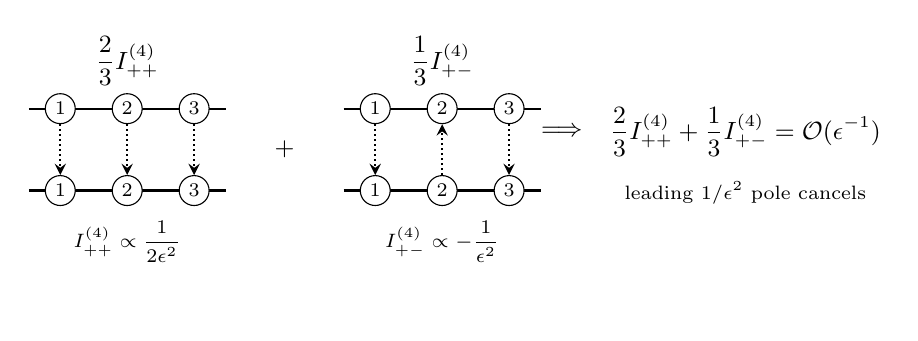
\begin{tikzpicture}[
    font=\small,
    op/.style={circle,draw=black!80!black,fill=white,inner sep=1.1pt,minimum size=0.38cm,font=\scriptsize},
    line/.style={draw=black!55!black,thick},
    ret/.style={densely dotted,draw=black!80!black,thick,->,>=stealth},
    adv/.style={densely dotted,draw=black!80!black,thick,->,>=stealth},
    arr/.style={->,draw=black!80!black,thick}
]
    \draw[line] (-0.25,0.52) -- (2.25,0.52);
    \draw[line] (-0.25,-0.52) -- (2.25,-0.52);
    \node[op] (a1) at (0.15,0.52) {1};
    \node[op] (a2) at (1.0,0.52) {2};
    \node[op] (a3) at (1.85,0.52) {3};
    \node[op] (b1) at (0.15,-0.52) {1};
    \node[op] (b2) at (1.0,-0.52) {2};
    \node[op] (b3) at (1.85,-0.52) {3};
    \draw[ret] (a1) -- (b1);
    \draw[ret] (a2) -- (b2);
    \draw[ret] (a3) -- (b3);
    \node[align=center,text=black!80!black] at (1.0,1.12)
        {\(\displaystyle \frac{2}{3}I^{(4)}_{++}\)};
    \node[align=center,font=\scriptsize,text=black!80!black] at (1.0,-1.17)
        {\(\displaystyle I^{(4)}_{++}\propto \frac{1}{2\epsilon^2}\)};

    \node at (3.0,0) {\(+\)};

    \draw[line] (3.75,0.52) -- (6.25,0.52);
    \draw[line] (3.75,-0.52) -- (6.25,-0.52);
    \node[op] (c1) at (4.15,0.52) {1};
    \node[op] (c2) at (5.0,0.52) {2};
    \node[op] (c3) at (5.85,0.52) {3};
    \node[op] (d1) at (4.15,-0.52) {1};
    \node[op] (d2) at (5.0,-0.52) {2};
    \node[op] (d3) at (5.85,-0.52) {3};
    \draw[ret] (c1) -- (d1);
    \draw[adv] (d2) -- (c2);
    \draw[ret] (c3) -- (d3);
    \node[align=center,text=black!80!black] at (5.0,1.12)
        {\(\displaystyle \frac{1}{3}I^{(4)}_{+-}\)};
    \node[align=center,font=\scriptsize,text=black!80!black] at (5.0,-1.17)
        {\(\displaystyle I^{(4)}_{+-}\propto -\frac{1}{\epsilon^2}\)};

    \node[text=black!80!black] at (6.52,0.23) {\(\Longrightarrow\)};
    \node[align=center,text=black!80!black] at (8.85,0.23)
        {\(\displaystyle
        \frac{2}{3}I^{(4)}_{++}
        +
        \frac{1}{3}I^{(4)}_{+-}
        =
        \mathcal O(\epsilon^{-1})\)};
    \node[align=center,font=\scriptsize,text=black!80!black] at (8.85,-0.55)
        {leading \(1/\epsilon^2\) pole cancels};

    \node[align=center,font=\scriptsize,text=black!80!black] at (3.0,-1.95)
        {};
\end{tikzpicture}
\caption{Causality-prescription diagrams for the IR-sensitive master integral. The Magnus/Murua weights assigned to the two oriented orderings cancel the leading \(1/\epsilon^2\) pole.}
\label{fig:eikonal-ir-causality}
\end{figure}
Nonetheless, in our computation of the eikonal phase in dCS theory, we find that the IR divergences cannot be removed by considering only the conservative sector. One might expect that including dissipative corrections would cancel these divergences. However, this expectation may be too naive: IR cancellation is a delicate procedure, and its realization may depend on theory-specific input. If the cancellation prescription is universal for a given class of theories, then this may not pose a serious obstruction. If, however, the prescription is theory dependent, it must be investigated carefully. In this thesis we do not attempt such an analysis, and instead leave the systematic treatment of this issue as an important direction for future work.}\\
Now, within this framework, with suitable care on $i\varepsilon$-prescription, observables are computed as one-point functions,
\begin{equation}
      \mathcal{O}(b_i,v_i)
      :=
      \langle\hat{\mathcal O}(\hat x,\hat h_{\mu\nu})\rangle_{\textrm{WQFT}}
      =
      \frac{1}{Z^{(n)}_{\textrm{WQFT}}}
      \int \mathcal{D}h_{\mu\nu}\,
      e^{iS_{EH}+iS_{gf}}
      \Big(\prod_{i=1}^{n}\mathcal{D}x_i\,e^{iS_{pm}^i}\Big)
      \mathcal O(x_i,h).
\end{equation}
For instance, the impulse and the waveform are obtained from
\begin{equation}
\begin{split}
    \Delta p_i^\mu
    &=
    m_i \int_{-\infty}^{\infty} d\tau_i\,
    \Big\langle \frac{d^2 z_i^\mu}{d\tau_i^2}\Big\rangle_{\text{WQFT}}
    =
    -m_i\omega^2\langle z_i^\mu(\omega)\rangle_{\text{WQFT}}\Big|_{\omega=0},\\
    f_h(k)
    &:=
    \frac{1}{4\pi m_p}\,
    \epsilon^\mu\epsilon^\nu\,
    k^2\langle h_{\mu\nu}(k)\rangle_{\textrm{WQFT}}\Big|_{k^2\to 0}.
\end{split}
\end{equation}
In practice, these one-point functions are evaluated perturbatively using tree-level WQFT diagrams. As in PM-EFT, one must exclude closed loops built solely from messenger and worldline propagators. In this way, WQFT provides an efficient route to classical observables, such as the impulse and waveform, within the framework of perturbative quantum field theory. In this thesis, we use these techniques to compute gravitational observables in several effective theories beyond General Relativity: scalar-tensor gravity, the phenomenological bottom-up EFT known as dynamical Chern-Simons theory, and Einstein-Maxwell-Dilaton theory, which arises as a low-energy effective theory of heterotic string theory.
\section{Celestial Amplitudes and Eikonalization}
{\color{black}
Beyond the study of observables in binary encounters, this thesis also explores the celestial dual of scattering amplitudes in higher-derivative theories of gravity, with particular emphasis on quadratic effective field theories. The motivation for this direction comes from the broader question of flat-space holography. The success of the AdS/CFT correspondence~\cite{Maldacena:1997re} shows that a theory of quantum gravity in an asymptotically anti-de Sitter spacetime can be equivalently described by a conformal field theory living on its boundary. It is therefore natural to ask whether an analogous holographic description exists for asymptotically flat spacetimes. In flat space, however, the most basic observables are not boundary correlation functions but scattering amplitudes defined at null infinity. This suggests that, if a holographic reformulation of flat-space quantum gravity exists, it should organize the usual momentum-space scattering amplitudes into observables of a lower-dimensional theory.

This idea is realized in the framework of Celestial Conformal Field Theory (CCFT)~\cite{Strominger:2013jfa,Strominger:2017zoo,Pasterski:2017ylz,Pasterski:2021raf,Donnay:2020guq}. In this approach, four-dimensional scattering amplitudes in asymptotically flat spacetime are mapped to conformal correlators on the celestial sphere at null infinity. The celestial sphere is the two-sphere of asymptotic null infinity, and each external massless particle is associated with a point on this sphere. The Lorentz group \(SL(2,\mathbb{C})\) acts on the celestial sphere as the global conformal group, while extensions of the asymptotic symmetry group are closely related to supertranslations and superrotations. Consequently, celestial amplitudes provide a bridge between three closely connected structures: flat-space scattering theory, asymptotic symmetries, and holography. This perspective has led to significant developments in the study of soft theorems, memory effects, and the conformal structure of scattering amplitudes~\cite{He:2014laa,Adamo:2019ipt,Gonzalez:2020tpi,Pasterski:2021fjn,Gonzo:2022tjm,Strominger:2021mtt}.

For massless scattering, an external particle is described by a positive energy \(\omega\) and a point \((z,\bar z)\) on the celestial sphere. The complex coordinate \(z\) is a stereographic coordinate on the sphere, and the corresponding null momentum can be parametrized as~\cite{Arkani-Hamed:2020gyp,Pasterski:2016qvg}
\begin{equation}
 p_\mu
 =
 \omega q_\mu(z,\bar z)
 =
 \frac{\omega}{\sqrt{2}}
 \left(
 1+|z|^2,\;
 z+\bar z,\;
 -i(z-\bar z),\;
 1-|z|^2
 \right).
\end{equation}
Here
\begin{equation}
 q_\mu(z,\bar z)
 =
 \frac{1}{\sqrt{2}}
 \left(
 1+|z|^2,\;
 z+\bar z,\;
 -i(z-\bar z),\;
 1-|z|^2
 \right)
\end{equation}
is a null vector specifying the direction of propagation of the particle. Thus the energy \(\omega\) fixes the overall scale of the momentum, while the celestial coordinates \((z,\bar z)\) fix its direction. In this parametrization the usual momentum-space data of each external massless particle are separated into an energy variable and an angular variable on the celestial sphere.

The celestial amplitude is obtained by Mellin transforming the momentum-space amplitude with respect to the external energies. For an \(n\)-point amplitude, one defines
\begin{equation}
    \mathcal{A}_n(\Delta_i,z_i,\bar z_i)
    =
    \int_0^\infty
    \prod_{i=1}^n
    d\omega_i\,\omega_i^{\Delta_i-1}\,
    \mathbb{M}_n(p_1,\ldots,p_n)\,
    \delta^{(4)}
    \left(
    \sum_{i=1}^n
    \epsilon_i\omega_i q_i
    \right),
\end{equation}
where \(q_i\equiv q(z_i,\bar z_i)\) is the null direction vector associated with the \(i\)-th point on the celestial sphere, and \(\omega_i>0\) is the corresponding energy. The sign \(\epsilon_i\) keeps track of whether the particle is outgoing or incoming:
\begin{equation}
    \epsilon_i =
    \begin{cases}
        +1, & \text{for an outgoing particle},\\
        -1, & \text{for an incoming particle}.
    \end{cases}
\end{equation}
The argument of the delta function is therefore the total four-momentum,
\begin{equation}
    \sum_{i=1}^n \epsilon_i p_i^\mu
    =
    \sum_{i=1}^n \epsilon_i \omega_i q_i^\mu,
\end{equation}
and the delta function imposes overall momentum conservation. The Mellin parameter \(\Delta_i\) is interpreted as the conformal dimension of the celestial operator associated with the \(i\)-th external particle. In this way, each external scattering state in four-dimensional momentum space is mapped to a conformal primary insertion on the celestial sphere.

For four-point scattering, the kinematics are especially simple because conformal symmetry fixes much of the coordinate dependence of the celestial correlator. The remaining nontrivial dependence can be expressed in terms of the conformal cross-ratio \(z\), together with its complex conjugate \(\bar z\). In physical scattering regions, momentum conservation imposes constraints on these variables, and different scattering channels correspond to different ranges of the cross-ratio. Thus the usual Mandelstam-channel structure of the momentum-space amplitude is translated into the analytic structure of the celestial correlator as a function of \(z\).
\begin{figure}
    \centering
    \includegraphics[width=0.6\linewidth]{Celestial.png}
    \caption{Celestial description of a four-dimensional scattering process. A momentum-space \(n\to m\) scattering amplitude in asymptotically flat spacetime is mapped, through a Mellin transform over the external energies, to a conformal correlator on the celestial sphere.}
    \label{fig23}
\end{figure}

After factoring out the universal kinematical dependence fixed by conformal covariance, the theory-dependent information is contained in a reduced Mellin amplitude. For a four-point process \(ij\to kl\), this reduced amplitude can be written schematically as
\begin{equation}
    \mathbfcal{A}^{ij\to kl}(\gamma,z)
    =
    B^{ij\to kl}(z)
    \int_0^\infty d\omega\,
    \omega^{\gamma-1}\,
    \mathbb{M}
    \big(
    s=\Phi(z)\omega^2,\;
    t=-\phi(z)\omega^2
    \big),
\end{equation}
where
\begin{equation}
    \gamma=\sum_{i=1}^4(\Delta_i-1).
\end{equation}
The functions \(\Phi(z)\) and \(\phi(z)\) are determined by the kinematic channel under consideration, while the prefactor \(B^{ij\to kl}(z)\) contains the universal dependence required by conformal symmetry and by the external quantum numbers. The reduced Mellin amplitude therefore isolates the dynamical content of the underlying four-dimensional theory. In particular, its analytic structure encodes information about the high-energy and fixed-angle behavior of the original momentum-space amplitude.

A central difficulty in celestial holography is that perturbative celestial amplitudes are often divergent when computed order by order in quantum field theory. These divergences arise because the Mellin transform probes both the low-energy and high-energy behavior of the momentum-space amplitude. In theories that are only effective descriptions, the ultraviolet behavior of the amplitude can lead to singularities or ill-defined Mellin integrals. One way to improve this behavior is to resum the perturbative expansion before performing the Mellin transform. This is particularly natural in the eikonal regime, where high-energy small-angle scattering amplitudes exponentiate. In General Relativity, eikonal exponentiation reorganizes the perturbative series and can lead to celestial amplitudes with improved analytic properties.

The inclusion of higher-derivative corrections makes this problem more subtle and more interesting. Quadratic curvature terms modify the momentum dependence of the gravitational amplitude and therefore alter the ultraviolet behavior that enters the celestial Mellin transform. From the celestial perspective, such corrections change the analytic structure of the Mellin amplitude and may soften some of the divergences that appear in pure Einstein gravity. At the same time, constructing the corresponding eikonal amplitudes becomes technically more involved, because higher-derivative interactions introduce additional momentum dependence and new scales into the problem. One of the goals of this thesis is to analyze these issues systematically for quadratic gravitational EFTs and to study how methods from analytic functional analysis can be used to characterize the resulting celestial amplitudes.}
\section{Computational Techniques and Methodology}
Even though QFT enters the classical two-body problem in many seemingly different ways, the technical core is the same. One organises the computation perturbatively and expresses the desired classical observables in terms of multidimensional loop-momentum integrals—Feynman integrals. As one pushes to higher orders, these integrals proliferate and develop increasingly rich analytic structure, which quickly becomes the main bottleneck to precision. This is why advances in amplitude methods and Feynman-integral technology tend to propagate across subfields: the same machinery that was refined for particle scattering now provides a common language connecting collider physics to classical gravitational dynamics.\par

The computation of Feynman Integrals is simplified by powerful algebraic structures. A general Feynman integral in momentum representation takes the form,
\begin{equation}
I \;=\; e^{\,l\epsilon\gamma_E}\,(\mu^2)^{\nu-\frac{lD}{2}}
\int \prod_{r=1}^{l}\frac{d^{D}\ell_r}{i\pi^{D/2}}
\prod_{j=1}^{n_{\text{int}}}\frac{1}{\bigl(q_j^{2}-m_j^{2}\bigr)^{\nu_j}}\,,
\tag{2.138}
\end{equation}
\noindent where
\begin{equation}
\epsilon=\frac{D_{\text{int}}-D}{2},
\qquad
\nu=\sum_{j=1}^{n_{\text{int}}}\nu_j,
\qquad
q_j=\sum_{r=1}^{l}\lambda_{jr}\ell_r+\sum_{r=1}^{n_{\text{ext}}-1}\sigma_{jr}p_r.
\tag{2.139}
\end{equation}
In standard introductory QFT courses, multiloop integrals are often introduced through the Feynman--Schwinger parameterisation. While this method is extremely useful, the integrals that arise in modern precision problems are frequently far more intricate: they depend nontrivially on kinematic invariants and the dimensional regulator $\epsilon$, and they appear in large families whose members proliferate rapidly with perturbative order. In such situations, it is neither practical nor conceptually efficient to evaluate each integral in isolation.  
\subsection*{Integration-by-Parts Identities}
A fundamental simplification in modern amplitude computations stems from the rich algebraic structure of Feynman integrals. The celebrated \textbf{Integration-by-Parts (IBP)} identities provide a systematic mechanism to relate thousands of seemingly distinct integrals within the same kinematic family. By exploiting these relations, an enormous system of integrals can be algebraically projected down to a finite, minimal basis of independent objects known as \textbf{Master Integrals} (MIs). This reduction is the algorithmic backbone of virtually all contemporary multi-loop calculations. The underlying principle relies on a core property of dimensional regularisation:
\begin{tcolorbox}[
  thesisstatementbox,
  title=Theorem,
  before skip=6pt,
  after skip=6pt,
  boxsep=2pt
]
%\restorethesisbodyformat
\textit{Within dimensional regularization, the integral of any total derivative with respect to a loop momentum strictly vanishes.}
\begin{equation}
    \int \prod_{r} d^d\ell_r\;
    \frac{\partial}{\partial \ell_i^\mu}
    \left(
      v^\mu
      \prod_{j}\frac{1}{D_j^{\nu_j}}
    \right)=0
\end{equation}
where the vector $v^\mu\in\{p_1,p_2,\ldots,p_{N_{\mathrm{ext}}},\ell_1,\ldots,\ell_r\}$, and the denominator factors are defined as $D_j=q_j^2-m_j^2$.
\end{tcolorbox}
%\restorethesisbodyformat

While a variety of highly optimised public codes (such as \textbf{\texttt{LiteRed}}\cite{Lee:2012cn}, \textbf{\texttt{Kira}}\cite{Maierhofer:2017gsa}, or \textbf{\texttt{FIRE}}\cite{Smirnov:2019qkx}) exist to generate and solve these IBP systems automatically, \textcolor{black}{ an important subtlety arises in the specific class of integrals relevant to computing scattering observables like impulse, waveform etc. These observables frequently feature \textbf{exponential factors} in the integrand. Sometimes, it is also a common understanding that treating the Fourier kernel as a part of the integral family may streamline the computation especially when we have massive loops  .}These exponentials modify the standard IBP relations in a way that is entirely invisible to conventional, rational-function-based automated generators. To illustrate this critical subtlety, consider a simple but nice integral family (The usefulness of incorporating the exponential factor into the IBP system was first pointed out in \cite{Brunello:2024ibk} in the context of computing the gravitational waveform in General Relativity.):
\begin{equation}
    I(a_1,a_2)
    =\int d^d\ell\,
    \frac{e^{D_1}}{D_1^{a_1}D_2^{a_2}},
    \qquad
    D_1=i\,\ell\!\cdot\! b,\quad
    D_2=\ell^2+m^2 .
\end{equation}
%\newpage
Applying the fundamental IBP theorem to this integrand yields:
\begin{equation}
\begin{split}
0
&=\int d^d\ell\,
\frac{\partial}{\partial \ell^\mu}
\left(
  \frac{v^\mu\,e^{D_1}}{D_1^{a_1}D_2^{a_2}}
\right)
\nonumber\\
&=\int d^d\ell\,
e^{D_1}\,
\frac{\partial}{\partial \ell^\mu}
\left(
  \frac{v^\mu}{D_1^{a_1}D_2^{a_2}}
\right)
\;+\;
\textcolor{brown}{
\int d^d\ell\,
\bigl(i\,v\!\cdot\! b\bigr)\,
\frac{e^{D_1}}{D_1^{a_1}D_2^{a_2}}
}\,.
\end{split}
\label{eq:exp-ibp-splitting}
\end{equation}
The \textcolor{brown}{second term} is the crucial new mathematical ingredient. It originates directly from the chain rule acting on the exponential $e^{D_1}$ and possesses no analogue in standard, purely rational IBP systems. By choosing specific vectors, such as $v^\mu=\ell^\mu$ and $v^\mu=b^\mu$, this derivative generates a coupled system of difference equations:
\begin{equation}
\begin{split}
&\left(-a_1-2a_2+d\right) I(a_1,a_2)
+2a_2 m^2\, I(a_1,a_2+1)
\textcolor{brown}{+I(a_1-1,a_2)}=0,
\\
&\textcolor{brown}{i b^2\, I(a_1,a_2)}
-i a_1 b^2\, I(a_1+1,a_2)
+2 i a_2\, I(a_1-1,a_2+1)=0.
\end{split}
\label{eq:exp-ibp-identities}
\end{equation}
Because widely used automated packages assume the integrand is a rational function of the loop momenta, they naturally reproduce only the uncoloured rational part of the splitting. The \textcolor{brown}{exponential-induced shift} must be manually injected into the system.
Once the complete IBP system is assembled, it can be solved iteratively using the Laporta algorithm. For modern, highly complex topologies, these custom systems are best tackled using finite-field arithmetic and sparse rational reconstruction techniques, such as those implemented in \textbf{\texttt{FiniteFlow}} (or via simple modifications to existing algebraic packages like \textbf{\texttt{LiteRed}}).
%\newpage
Below is an illustrative snippet demonstrating how to define and solve this modified, exponentially-shifted IBP system using \texttt{FiniteFlow}:

\begin{lstlisting}[language=Mathematica, caption={Solving simple IBPs using FiniteFlow}, label={lst:finiteflow-ibp}]
<< FiniteFlow`
Eq1[a1_, a2_] := (d - 2*a2 - a1)*I[a1, a2] + I[a1-1, a2] + 2*a2*m^2*I[a1, a2+1] == 0
Eq2[a1_, a2_] := bSq*I[a1, a2] + 2*a2*I[a1-1, a2+1] - a2*bSq*I[a1+1, a2] == 0

SeedEqs = Flatten[Table[{Eq1[a1, a2], Eq2[a1, a2]},
  {a1, -2, 1}, {a2, 0, 6}]];
allIntegrals    = DeleteDuplicates[Cases[SeedEqs, _I, Infinity]];
orderedIntegrals = Reverse[SortBy[allIntegrals,
  {Abs[#[[1]]] + Abs[#[[2]]] &, Abs[#[[2]]] &}]];
targets = {I[0, 4]};
solution = FFSparseSolve[SeedEqs, orderedIntegrals,
  "Parameters" -> {d, m, bSq}, "NeededVars" -> targets,
  "MaxPrimes" -> 150, "MaxDegree" -> 500] /. bSq -> b^2;

Print["=== Solution ==="];
Print[solution];
\end{lstlisting}
By solving this system, the infinite tower of integrals collapses. For this specific family, one is left with exactly three Master Integrals: $I(1,0)$, $I(1,1)$, and $I(2,0)$. In general, for any given $L$-loop topology with a defined set of external momenta, \textbf{any} Feynman integral $\mathcal{I}$ within that family can be uniquely expanded as a linear combination of its basis Master Integrals $\mathcal{M}^{(k)}_{\mathrm{MI}}$:
\begin{equation}
   \mathcal{I}=\sum_k c_k(d,s_{ij}) \mathcal{M}^{(k)}_{\mathrm{MI}}
\end{equation}
where the IBP reduction coefficients $c_k(d,s_{ij})$ are strictly rational functions of the spacetime dimension $d$ and the kinematic invariants $s_{ij}=p_i\cdot p_j$.

With the IBP reduction complete, the formidable task of evaluating thousands of individual loop integrals is entirely bypassed. The challenge is now distilled down to its purest form: evaluating just the basis set of Master Integrals. One efficient way to compute the master integral is the method of differential equations. This technique is primarily more useful when the Feynman integrals do not have non-perturbative factorisation in the dimensional regularisation parameter $\epsilon$ and kinematic factors $s,t,u,m^2$. Let's also discuss these techniques (with a simple toy example). Let $\vec{\mathbfcal{J}}=(J_1,J_2,\ldots,J_n)$ denote the vector of Master Integrals (MIs), which in general depend on the set of kinematic invariants
$\boldsymbol{X}$ as well as on the spacetime dimension $d$. Differentiating with respect to $\boldsymbol{X}$ and subsequently applying IBP reduction
ensures that these derivatives can be expressed again as linear combinations of the same master integrals, and they satisfy the following homogeneous system of matrix differential equations.
\begin{equation}
    \partial_{x}\vec{\mathbfcal{J}}=\Omega_{x}\vec{\mathbfcal{J}}\,.
\end{equation}
 Collecting all differentials, one can write the
differential 1-form,
\begin{equation}
    d\vec{\mathbfcal{J}}=\boldsymbol{\Omega}\cdot\vec{\mathbfcal{J}},\qquad \boldsymbol{\Omega}=\sum_{x\in \boldsymbol{X}}\Omega_xdx\,.\label{7}
\end{equation}
By choosing an ordering in which master integrals associated with simpler sub-topologies (with a lesser number of denominators ) are placed first, the differential-equation system can often be arranged into a (block) lower-triangular form. Consistency of the differential system is then encoded in the integrability condition $d^2\vec{\mathbfcal{J}}=0$, which translates into the flatness (Maurer--Cartan) equation for the connection one-form,
\begin{equation}
d\boldsymbol{\Omega}=\boldsymbol{\Omega}\wedge\boldsymbol{\Omega}\, .
\end{equation}
The solution of the differential equation can be formally expressed as a path-ordered integral,
\begin{equation}
    \begin{split}
        \vec{\mathbfcal{J}}(\boldsymbol{x},\epsilon)=\mathcal{P}\exp\left(\int d\boldsymbol\Omega(\boldsymbol{x},\epsilon)\right) \vec{\mathbfcal{J}}(\boldsymbol{x}_0,\epsilon)\label{9}
    \end{split}
\end{equation}
where $\vec{\mathbfcal{J}}(x_0,\epsilon)$ is the vector of the mater integrals determined at a particular kinematic point, sometimes known as the boundary integrals. The boundary integrals can usually be computed using the elementary techniques of evaluating Feynman integrals, such as Feynman and Schwinger parametrisation. However, directly computing the path-ordered integral in \eqref{9} is quite cumbersome, as it is very difficult to determine the order of $\epsilon$. It is possible to make a change of basis from $\vec{\mathbfcal{J}}$ to $\vec{\mathbfcal{H}}$ : $\vec{\mathbfcal{H}}=\mathbf{T}\cdot \vec{\mathbfcal{J}}$, where $\mathbf{T}$ is a $n\times  n$ basis transformation matrix. Therefore, the transformed basis of MIs satisfies a transformed set of differential equations,
\begin{equation}
d\vec{\mathbfcal{H}}=\widetilde{\boldsymbol{\Omega}}\cdot\vec{\mathbfcal{H}},\qquad  \widetilde{\boldsymbol{\Omega}}=\mathbf{T}\cdot \boldsymbol{\Omega}\cdot \mathbf{T}^{-1}-\mathbf{T}d\mathbf{T}^{-1}\,.
\end{equation}
It was conjectured in \cite{Henn:2013pwa} that there exist a particular choice of basis transformation such the the transformed differential equation has $\epsilon$-factorized form: $d\vec{\mathbfcal{H}}=\epsilon\,d{\hat{\boldsymbol{\Omega}}}\cdot\vec{\mathbfcal{H}}$, where, $d{\hat{\boldsymbol{\Omega}}}$ has only logarithmic singularities and can be written in $d\log$-form: $d{\hat{\boldsymbol{\Omega}}}=\sum_{\eta_i\in A}M_i\,d\log\eta_i$, where, $\eta_i$ are called letters, and they only encodes the kinematic dependence of the differential equations, their collection is called Alphabet $A$, and $M_i$ are constant rational matrices. This particular choice of basis is called the canonical basis. The systematic construction of such a basis can be achieved via the Lee algorithm \cite{Lee:2014ioa}. In practice, this complex algebraic transformation is now heavily (semi-)automated and readily available through several specialized public computer algebra packages, including \textbf{\texttt{Libra}} \cite{Lee:2020zfb}, \textbf{\texttt{Canonica}} \cite{Meyer:2017joq}, \textbf{\texttt{Fuchsia}} \cite{Gituliar:2017vzm}, and \textbf{\texttt{INITIAL}} \cite{Dlapa:2020cwj}. In canonical basis, the path order integral can be expanded in a Laurent expansion of $\epsilon$, formally,
\begin{equation}
    \vec{\mathbfcal{H}}=\left(\mathbb{I}+\epsilon\int_{\gamma} d\hat{\boldsymbol{\Omega}}+\epsilon^2\int_{\gamma}d\hat{\boldsymbol{\Omega}}\cdot d\hat{\boldsymbol{\Omega}}+\cdots\right)\vec{\mathbfcal{H}}_0
\end{equation}
\begin{figure}
    \centering
\includegraphics[width=0.25\linewidth]{Sphere1.jpeg}
    \caption{Geometry and contour of nested integrals}
    \label{sp1}
\end{figure}
Each order of an iterated integral corresponds to the successive integration of logarithmic differential 1-forms. Given an alphabet of such forms, typically defined as $\omega_a = d\log(z - a)$, the iterated integral of a sequence of these letters along a specified continuous contour $\gamma$ is expressed as:
\begin{equation}
    \int_{\gamma} \omega_{a_1} \circ \cdots \circ \omega_{a_n}=\int_{\gamma_1}\frac{dz_1}{z_1-a_1}\int_{\gamma_2}\frac{dz_2}{z_2-a_2}\int_{\gamma_3}\frac{dz_3}{z_3-a_3}\cdots,\quad \gamma_i(0)=0,\,\gamma_i(1)=t_{i-1},\, a_i=\{0,1,\sigma_j\}
\end{equation}
Evaluating these iterated integrals with simple logarithmic kernels gives rise to a rich space of functions known as Generalised Polylogarithms (G-MPLs), or Multiple Polylogarithms. Geometrically, these functions are most naturally defined on the \textbf{punctured Riemann sphere}, $\mathbb{C} \cup \{\infty\}$ (see Fig.~(\ref{sp1})). The ``punctures'' on this sphere correspond precisely to the simple poles of the rational logarithmic kernels---the specific points $a_i$ where the differential forms become singular. 
By framing this space on the compact Riemann sphere rather than the open complex plane, the point at infinity is treated on equal footing with the finite singularities. Because the differential 1-forms are closed, the specific value of the resulting GPL is determined entirely by the homotopy class of the integration path $\gamma$. The sphere provides a complete topological canvas for tracking how this contour winds around the singular punctures, elegantly capturing the branch cuts and monodromy properties of the integrals.
To truly appreciate the power of the differential equation method, we must recognise how it shifts the paradigm of computing Feynman integrals. Instead of brute-forcing complicated momentum integrations over massive propagators, this technique transforms the problem into a highly systematic exercise in linear algebra and the analytic continuation of topological paths.
Let us see this in action through an elegant example.


\textbf{The Setup: From Integrals to Algebra.}
Consider the family of two-loop Feynman integrals associated with a Sunrise-type topology with one massive internal line. The integral family is defined as:
\begin{equation}
  J_{a_1,...,a_5}=\begin{minipage}
          [h]{0.40\linewidth}
	\vspace{1.2 pt}
	\scalebox{0.6}{\includegraphics[width=\linewidth]{sunrise.png}}
      \end{minipage} \hspace{-2 cm}= \int d^d\ell_1 d^d\ell_2 \frac{1}{D_1^{a_1}D_2^{a_2}D_3^{a_3}D_4^{a_4}D_5^{a_5}}
\end{equation}
where the inverse propagators are $D_1=\ell_1^2-m^2$, $D_2=\ell_2^2$, $D_3=(p-\ell_1-\ell_2)^2$, $D_4=(p-\ell_1)^2$, and $D_5=(p-\ell_2)^2$, with the kinematic invariant $p^2=s$. 

Directly integrating this for general powers $a_i$ is exceptionally difficult. However, by leveraging Integration-By-Parts (IBP) identities, the infinite-dimensional space of these integrals is algebraically reduced to a finite set of just seven Master Integrals (MIs):
\begin{equation}
\begin{split}
    \vec{\mathbfcal{J}} = &\{J_{0,0,1,1,1}, J_{1,0,1,0,1}, J_{1,1,0,0,1}, J_{1,1,1,0,0}, J_{2,1,1,0,0}, J_{1,0,1,1,1}, J_{1,1,0,1,1}\}
    \end{split}
\end{equation}
\textbf{The Differential Equation.}
Instead of integrating, we differentiate. Taking the derivative of these MIs with respect to the dimensionless kinematic invariant $x = \frac{s}{m^2}$ yields a closed, coupled system of first-order differential equations:
\begin{equation}
    \partial_{x}\vec{\mathbfcal{J}} = \Omega(x,\epsilon)\cdot \vec{\mathbfcal{J}}
\end{equation}
where the matrix $\Omega(x,\epsilon)$ governs the system's dynamics:
\begin{equation}
\Omega(x,\epsilon) = \left(
\begin{array}{ccccccc}
 \frac{1-2 \epsilon }{x} & 0 & 0 & 0 & 0 & 0 & 0 \\
 0 & 0 & 0 & 0 & 0 & 0 & 0 \\
 0 & 0 & -\frac{\epsilon }{x} & 0 & 0 & 0 & 0 \\
 0 & 0 & 0 & \frac{1-2 \epsilon }{x} & -\frac{1}{x} & 0 & 0 \\
 0 & 0 & 0 & \frac{-6 \epsilon ^2+7 \epsilon -2}{(x-1) x} & \frac{2-(x+3) \epsilon }{(x-1) x} & 0 & 0 \\
 \frac{2-3 \epsilon }{(x-1) x} & \frac{\epsilon -1}{(x-1) x} & 0 & 0 & 0 & \frac{1-(x+1) \epsilon }{(x-1) x} & 0 \\
 0 & 0 & \frac{\epsilon -1}{(x-1) x} & 0 & 0 & 0 & \frac{1-2 x \epsilon }{(x-1) x} \\
\end{array}
\right)
\end{equation}
Notice that in this raw form, the kinematic dependence (the variable $x$) and the dimensional regulator (the variable $\epsilon$) are deeply entangled. Solving this directly remains non-trivial.

\textbf{The Breakthrough: The Canonical Basis.}
This is where the true power of the method emerges. By finding a highly specific algebraic transformation $\mathbf{T}$, we can rotate our basis of MIs from $\vec{\mathbfcal{J}}$ to a ``canonical basis'' $\vec{\mathcal{H}}$, defined by $\vec{\mathcal{H}} = \mathbf{T}\cdot \vec{\mathbfcal{J}}$. For this system, the transformation matrix is:
% Preamble:
% \usepackage{graphicx}
\begingroup
\setlength{\arraycolsep}{3pt}
\renewcommand{\arraystretch}{1.15}
\begin{equation}
\mathbf{T} =
\resizebox{\textwidth}{!}{$
\begin{pmatrix}
\dfrac{28x(2\epsilon^2-\epsilon)}{5(9\epsilon^2-9\epsilon+2)} & 0 & 0 & 0 & 0 & 0 & 0 \\
0 & -\dfrac{3(2\epsilon-1)}{5(\epsilon-1)} & 0 & 0 & 0 & 0 & 0 \\
0 & 0 & \dfrac{3(2\epsilon-1)}{5(\epsilon-1)} & 0 & 0 & 0 & 0 \\
0 & 0 & 0 & \dfrac{8\epsilon}{9\epsilon^2-9\epsilon+2}\!\left(x-\dfrac{1}{x}\right) &
\dfrac{4(5x\epsilon+7\epsilon-2)}{9\epsilon^2-9\epsilon+2}-\dfrac{16\epsilon}{x(9\epsilon^2-9\epsilon+2)} & 0 & 0 \\
0 & 0 & 0 & \dfrac{8\epsilon}{3\epsilon-1}\!\left(\dfrac{1}{x}-1\right) &
\dfrac{16\epsilon}{x(3\epsilon-1)}-\dfrac{4(8\epsilon-1)}{3\epsilon-1} & 0 & 0 \\
-\dfrac{8}{5x}-\dfrac{4(\epsilon+2)}{5(3\epsilon-1)} & -\dfrac{3}{5x} & 0 & 0 & 0 & \dfrac{1}{x}-1 & 0 \\
0 & 0 & \dfrac{3}{5x} & 0 & 0 & 0 & 1-\dfrac{1}{x}
\end{pmatrix}
$}
\end{equation}
\endgroup
Applying this transformation achieves \textbf{$\epsilon$-factorization}. The new, transformed differential equation takes a remarkably beautiful and simple form, expressed in terms of logarithmic differential 1-forms:
\begin{equation}
    d\vec{\mathcal{H}} = \epsilon \, \hat{\Omega}_{x} \vec{\mathcal{H}}
\end{equation}
where the connection $\hat{\Omega}_{x}$ separates cleanly into constant matrices weighted by pure $d\log$ forms:
\begin{align}
\hat{\Omega}_{x} = \left(
\begin{array}{ccccccc}
 -2 & 0 & 0 & 0 & 0 & 0 & 0 \\
 0 & 0 & 0 & 0 & 0 & 0 & 0 \\
 0 & 0 & -1 & 0 & 0 & 0 & 0 \\
 0 & 0 & 0 & -3 & -6 & 0 & 0 \\
 0 & 0 & 0 & 2 & 4 & 0 & 0 \\
 -\frac{24}{5} & -\frac{3}{5} & 0 & 0 & 0 & 1 & 0 \\
 0 & 0 & -\frac{3}{5} & 0 & 0 & 0 & 0 \\
\end{array}
\right) d\log(x) + \left(
\begin{array}{ccccccc}
 0 & 0 & 0 & 0 & 0 & 0 & 0 \\
 0 & 0 & 0 & 0 & 0 & 0 & 0 \\
 0 & 0 & 0 & 0 & 0 & 0 & 0 \\
 0 & 0 & 0 & -4 & -9 & 0 & 0 \\
 0 & 0 & 0 & 0 & 0 & 0 & 0 \\
 \frac{44}{5} & \frac{3}{5} & 0 & 0 & 0 & -2 & 0 \\
 0 & 0 & \frac{3}{5} & 0 & 0 & 0 & -2 \\
\end{array}
\right) d\log(x-1)
\end{align}
\textbf{The Power of Transport:}
Because $\epsilon$ is factored out, the solution to this matrix differential equation is immediately given as a Dyson series of iterated integrals. The canonical Master Integrals simply possess a Laurent expansion in $\epsilon$:
\begin{equation}
\begin{split}
    \vec{\mathcal{H}} &= \left( \mathbb{I} + \epsilon \int_{\gamma} \hat{\Omega}_x + \epsilon^2 \int_{\gamma} \hat{\Omega}_x \circ \hat{\Omega}_x + \mathcal{O}(\epsilon^3) \right) \vec{\mathcal{H}}_\infty \\ 
    &= \left( \mathbb{I} + \epsilon \sum_{a_i \in \{0,1\}} M_{a_i} \int_{\gamma} d\log(x-a_i) + \epsilon^2 \sum_{a_i, a_j \in \{0,1\}} M_{a_i} M_{a_j} \int_{\gamma} d\log(x-a_i) \circ d\log(x-a_j) + \cdots \right) \vec{\mathcal{H}}_{\infty}
\end{split}
\end{equation}
\textit{This is the ultimate triumph of the method.} The difficult integration over physical space-time momenta has been entirely replaced by a set of nested integrals. Moreover, the boundary vector $\vec{\mathcal{H}}_\infty$ can be evaluated at a kinematically simple point. By taking the Regge limit ($s \to \infty$) or the massless limit ($m \to 0$), the originally formidable massive integrals become trivial to compute (However, one needs to be precise about the regions while expanding  for boundary data; we will discuss these in great detail in the next chapter). The iterated integrals of the $d\log$ forms then seamlessly analytically continue, or transport, this trivial massless result back to the massive kinematic regime. We have effectively computed a complex, massive, multi-loop integral simply by evaluating its simpler massless counterpart and reading the geometric structure of its singularities. In general, different classes of special functions may appear in the computation of Feynman integrals, especially for higher loop computations. To systematically identify the precise class of functions spanned by the final solution, it is highly effective to stratify the family of master integrals into its constituent topological sectors. Because the associated system of differential equations inherently possesses a block-triangular structure, the homogeneous component (usually some non-homogeneous part may be present, which comes from lower sub-topologies) of each diagonal block uniquely dictates the functional alphabet required to evaluate that specific sector. By isolating a specific $k \times k$  block of the homogeneous differential equation system, one can equivalently recast the dynamics of a chosen Master Integral, $J_i$, into a single $k$-th order scalar differential equation:
\begin{equation}
    \mathcal{L}_k J_i(x) = 0, \qquad \mathcal{L}_{k} = \frac{d^k}{dx^k} + \sum_{j=0}^{k-1} c_j(x)\frac{d^j}{dx^j}
\end{equation}
Here, the coefficients $c_j(x)$ are purely rational functions of the kinematic variable $x$. The differential operator $\mathcal{L}_k$ defines the Picard-Fuchs (PF) equation, and its factorisation properties elegantly encode the underlying algebraic geometry of the Feynman integral. 
The structure of this factorisation directly dictates the functional alphabet required to express the solution:
\begingroup
%\restorethesisbodyformat
\setlength{\tabcolsep}{0pt}
\renewcommand{\arraystretch}{1.5} % Increased stretch for better vertical spacing between rows
\begin{center}
\begin{tabularx}{0.94\linewidth}{@{}>{\raggedright\arraybackslash}m{0.78\linewidth}@{\hspace{1.2em}}>{\centering\arraybackslash}m{0.16\linewidth}@{}}

\textbf{Genus-0 rational curve $\implies$ Multiple Polylogarithms.} If the PF operator factorizes entirely into first-order components, such that $\mathcal{L}_{k} = \mathcal{L}_1^{(1)} \circ \mathcal{L}_1^{(2)} \circ \cdots \circ \mathcal{L}_1^{(k)}$, with each $\mathcal{L}_1^{(m)} = \left(\frac{d}{dx} - r_m(x)\right)$, the solution space is strictly spanned by Generalized Multiple Polylogarithms (G-MPLs) and standard iterated integrals. &
\includegraphics[width=\linewidth]{Sphere.png}
\\
\textbf{Genus-1 (or torus) irrational curve (Elliptic curve) $\implies$ Elliptic polylogarithms.} If the operator cannot be fully reduced and leaves behind irreducible second-order factors, the geometry transcends simple poles. The corresponding solutions are governed by elliptic curves, requiring integrals over elliptic kernels. &
\includegraphics[width=\linewidth]{Torus.png}
\\ 
\textbf{Higher genus irrational curves $\implies$ Calabi-Yau periods .} Higher-order irreducible components signal the presence of profoundly more complex geometric structures within the scattering amplitude, such as CY3 surfaces or more general Calabi-Yau manifolds. &
\includegraphics[width=\linewidth]{K3.png}
\end{tabularx}
\end{center}
\endgroup
\textit{Throughout the remainder of this thesis, we will focus exclusively on Feynman integrals whose Picard-Fuchs operators completely factorise at first order, thereby restricting our analytic evaluations entirely to the simplest class: Generalised Multiple Polylogarithms.}
\\
This functional hierarchy provides the organising lens for the technical chapters that follow.
%\newpage
\section{Thesis in a nutshell}
\noindent A chapter-wise summary of the thesis is as follows.
\begin{itemize}[leftmargin=1.75em,topsep=0pt,itemsep=0.18em,parsep=0pt,partopsep=0pt]
  %\item \textbf{\texttt{Chapter 1. Introduction.}} This chapter is devoted to a detailed introduction to the context, motivation, and main goals of the thesis. We discuss the various field-theoretic methods that form the backbone of the analyses in the subsequent chapters, and comment on some of their advantages as well as their limitations. Since Feynman integrals play a central role in many of the computations presented in this thesis, we also introduce this subject and briefly review some of the modern techniques used to evaluate them. Along the way, we highlight their connections with seemingly distant areas of mathematics, such as algebraic geometry. We conclude the chapter with a chapter-by-chapter overview of the thesis and a summary of the main results.

  \item \textbf{\texttt{Chapter 2. WEFT of Black-Hole Binaries with Dark Photon and Axion.}} In this chapter, we investigate the correction to the potential that gives rise to the bound orbits and radiation from non-spinning inspiralling binary black holes in a dark matter environment consisting of \textit{axion-like particles} and \textit{dark photons} using the techniques of \textit{Worldline Effective Field Theory}. We compute the conservative dynamics up to $1$PN order for gravitational, electromagnetic, and Proca fields and up to $2$PN order for the scalar field. The effect of axion-electromagnetic coupling ($g_{a\gamma\gamma}$) arises in the conservative dynamics at $2.5$PN order and the kinetic mixing constant ($\gamma$) at $1$PN order. Furthermore, we calculate the radiation due to the various fields present in our theory. We find that the contribution of $g_{a\gamma\gamma}$ to the gravitational radiation appears at $N^{(7)}LO$ and to the scalar radiation at $N^{(5)}LO$. We also find that these radiative corrections due to the coupling $g_{a\gamma\gamma}$ vanish for any orbit confined to a plane because of the existence of a \textit{binormal}-like term in the effective radiative action, but give rise to non-zero contributions for any orbit that lies in \textit{three dimensions}. Last but not least, $\gamma$ contributes to the gravitational radiation at $N^{(2)}LO$ and $N^{(4)}LO$.

  \item \textbf{\texttt{Chapter 3. Classical Black-Hole Scattering in Scalar-Tensor Gravity from WQFT.}} In this chapter, we move to the problem of computing observables in classical black-hole scattering in the context of the simplest modification of General Relativity, namely scalar-tensor gravity. We compute the two observables, impulse and waveform, in a non-spinning black-hole scattering event for the scalar-tensor theory of gravity with a generic scalar potential using the techniques of Worldline Quantum Field Theory. We mainly investigate corrections to the above-mentioned observables arising from the extra scalar degree of freedom. For the computation of the impulse, we consider the most general scenario by making the scalar field massive and then show that each computed diagram has a smooth massless limit. We compute the waveforms for a scalar and a graviton up to 2PM, treating the scalar as massless. Furthermore, we discuss the case in which the scalar has mass and how the radiation integrals become more involved than in the massless case. We also obtain analytical results using the stationary-phase approximation.

  \item \textbf{\texttt{Chapter 4. Spinning Two-Body Problem in dCS Gravity Using WQFT.}} In this chapter, we extend the analysis to the case of spinning black holes in dynamical Chern-Simons gravity. Our main objective is to compute the WQFT partition function, or equivalently, the eikonal phase, for black-hole scattering in this theory using the methods of spinning worldline quantum field theory. We consider the scattering of spinning compact objects and explain in detail the ingredients required to construct the partition function. A central part of the computation involves the evaluation of the relevant two-loop integrals. For this purpose, we derive the $\epsilon$-expansion of the necessary master integrals using Integration-by-Parts (IBP) reduction together with differential equation techniques. These results are then used to determine the eikonal phase at linear order in spin up to third post-Minkowskian (3PM) order. We also analyse how the phase depends on the relative orientations of the black-hole spins, which is crucial for the structure of the resulting observables, since the eikonal phase serves as the basic generating quantity for the classical dynamics. In addition, we discuss the role of asymptotic supersymmetry in the worldline degrees of freedom, which provides a natural way to define the spin of black holes even in the presence of additional propagating fields, such as the dilaton, in addition to the usual massless spin-two graviton. We also comment on the infrared issues that arise in this context and discuss their possible origins and resolutions.

  \item \textbf{\texttt{Chapter 5. Heterotic Footprints in Classical Gravity.}} In this chapter, in a complementary direction, we use amplitude-based approaches to study classical scattering of charged black holes in Einstein-Maxwell-Dilaton (EMD) theory. Working in the classical (Post-Minkowskian) regime, we extract the conservative two-body potential by expanding the one-loop amplitudes in the soft regime. We explicitly show that, as in GR, the relevant soft amplitudes are infrared (IR) finite when long-range interactions are consistently treated via the Lippmann-Schwinger equation and the associated IR subtraction. The scattering angle is then obtained from the eikonal exponentiation of the soft amplitude. Our results track the separate roles of electromagnetic and dilatonic charges in both the conservative dynamics and the eikonal phase, and they smoothly reduce to the GR limit when the charges and the dilaton coupling are switched off. Where applicable, we compare our results with existing literature and find agreement. These findings provide amplitude-based benchmarks for compact-object dynamics in EMD and furnish building blocks for waveform modelling in beyond-GR scenarios.

  \item \textbf{\texttt{Chapter 6. Celestial Amplitude, Shadow, and OPE in Quadratic Gravity.}} In this chapter, as a further investigation into higher-derivative effective field theories, we compute the celestial amplitude arising from higher-curvature corrections to Einstein gravity, incorporating phase dressing. The inclusion of such corrections leads to effective modifications of the theory's ultraviolet (UV) behaviour. In the eikonal limit, we find that, in contrast to Einstein gravity, where the $u$- and $s$-channel contributions cancel, these contributions remain non-vanishing in the presence of higher-curvature terms. We examine the analytic structure of the resulting amplitude and derive a dispersion relation for the phase-dressed eikonal amplitude in quadratic gravity. Furthermore, we investigate the celestial conformal block expansion of the Mellin-transformed conformal shadow amplitude within the framework of celestial conformal field theory (CCFT). As a consequence, we compute the corresponding operator product expansion (OPE) coefficients using the Burchnall-Chaundy expansion. In addition, we evaluate the OPE via the Euclidean OPE inversion formula across various kinematic channels and comment on its applicability and implications. Finally, we briefly explore the Carrollian amplitude associated with the corresponding quadratic EFT.
\end{itemize}
